\chapter{Background}
\label{ch:background}

Formal methods are a specific type of mathematical notation which is based on the techniques of the specification, verification and development of software and hardware systems \cite{whatareformalmethods}. Since our thesis presents \gls{zmath} we go right to the beginning of the framework, to describe how mathematical notation came about. Then we describe the original MathLang framework (the framework which \gls{zmath} is an adaptation of) and then give the reader an idea of other formal methods and languages. In the next section we wish to describe what is the language of Z and give more details of it's syntax and semantics. We then highlight other proving techniques which have been done for maths, formal methods and Z.

\section{Mathematical Notations}

Computer science (and thus computer systems) have evolved from basic mathematics. We can say that formal specification writers are practising mathematicians as they write system specifications in a formal manner. Therefore we must start right at the beginning at the foundation of mathematical notation.

\subsection{Right from the beginning}
\label{subsec:rftb}

The relationship between mathematical reasoning and practising mathematicians started out early on during the ancient Greeks where logic was already being studied. Reasoning in logic was used for just about anything not just mathematics such as law, medicine and farming. This very early form of mathematics made very famous discoveries such as Aristotles logic \cite{aristotle}, Euclid's geometry \cite{euclid} and Leibniz Calculus \cite{leibniz}.

Further on in the 1800's, Frege wrote \emph{Die Grundlagen der Arithmetik} \cite{frege} and other works where he noted that mathematics is a branch of logic. In this works, he began building a solid foundation for mathematics. This early foundation along with Cantors set theory \cite{cantor} was argued to be inconstant and thus Russel found a paradox in this work.

In the late 19th century and beginning of 20th century, Russell \& Whitehead \cite{whitehead1912principia} started to form a basis for mathematical notation. Their three volume work describes a set of rules from which all mathematical truths could be proven. In these early stages the authors try to derive all maths from logic. This ambitious project was the first stepping stone in collaborating all mathematics under one notation.

Further to Russell \& Whitehead's work, Bourbanki \footnote{A name given to a collective of mathematicians} wrote a series of books beginning n the 1935's with the aim of grounding mathematics. Their main works is included in the Elements of Mathematics series \cite{opac-b1128208} which does not need any special of knowledge of mathematics. It describes mathematics from the very beginning and goes through core mathematical concepts such as set theory, algebra, function etc. and gives complete proofs for these concepts.

Adding to Russell's work, Zermelo introduced an acclimatisation of set theory which was later extended by Frankel and Skolem to form ZF set theory \cite{zfc}. This new theory is what we will later see the Z notation is based on and the notation this thesis checks the correctness of.

\subsection{Computerisation of Maths and Proof Systems}

In the 21st century, a great area of research is how use, store and support this mathematical knowledge. Since automation has become more and more used, mathematicians have looked into ways in which they can use computers to reason about and provide services to mathematics. This would include all areas of mathematics, such as logic, mechanics and software specifications. Mathematical knowedge can be represent in lots of different ways including the following:

\begin{itemize}
\item One can typeset mathematics into a computer using a system such as \LaTeX{} \cite{latex} . These systems can edit and format mathematical knowledge so that it can be stored or printed. These systems provide good visual appearance and thus can be used for storing and archiving ones documents. Even Z specification, have their own package for \LaTeX{} and thus the structure of the specification can be represented both formally and informally. However, it is difficult to represent the logical structure of mathematical formulas and the logical structure of mathematics is embedded in natural language. Therefore, there isn't a lot of support for checking the correctness of general mathematics represented in the system (Z specifications on their own can be checked but this is discussed further in section \ref{subsec:provingSystemsForZ}).

\item Systems such as proof assistants (e.g. Isabelle \cite{isabelle}, Coq \cite{coq} and ProofPower-Z \cite{pp}) and automated theorem provers (e.g. Boyer-Moore, Otter) and jointly called proof systems. Proof systems each provide a formal language for writing mathematics. Early work on proof systems was done by De Bruijn when he worked on the AutoMath \cite{selectedautomath} project. AutoMath (automating mathematics) was the first attempt to digitize and formally prove mathematics which was assisted by a computer. AutoMath is described as a language for formalising mathematical texts and for automating the validation of mathematics. The AutoMath project is what brought uniform notations and automated proof together.

Further to this work, there has been many other proof systems implemented to implement and check mathematics for total correctness. It is possible to access the semantics of mathematics in these systems. However, with these proof systems, a user must choose a specific proof system and one of these have their advantages and disadvantages. Also, each of these proof systems also take quite some time to learn. There is much documentation on some of these systems (e.g. Isabelle) and some are very well supported. But this in turn can be a downfall, as there is so much documentation, it is difficult to know how much one must learn and where to start. The best way of learning one of these system is from someone who already is an expert in the chosen proof system. A lot of the proof systems use proof tactics to constructs proofs and make them smaller, however to prove certain properties in a proof system, one can use various tactics to get to the same goal and may sometimes be difficult to find which tactic is best to use.

With these disadvantages many academic and industrial mathematicians do not generally use the mathematics written in the language of the proof system and usually are not willing to spend the time to check the correctness of their own work in this system.

\item There also exists semantical oriented document representations like OpenMath \cite{openmath} and OMDoc \cite{omdoc}. These systems are better than the typesetting systems such as \LaTeX{} to produce readable and printable version of the mathematical knowledge written. Some aspects of the semantics of the mathematics can be represented in these type systems. However, when using these systems it is difficult to control the presentation and therefore a typesetting system is more likely to be used. Like the typesetting system, systems like OMDoc also have difficult reading the logical structure of mathematics embedded in the natural language of the text. Systems like OMDoc can associate symbolic formulas with chunks of natural language text, however these chunks can not be seen by the computer and thus can not be checked if it is correct.

Another disadvantage is that although there is support for the semantics of the mathematics, these systems can not support the semantics in terms of logical foundations for mathematics (unlike proof systems).
\end{itemize}


\subsection{Conclusion}

In summary the \gls{math} framework has been developed to be used as a bridge between the categories mentioned above as a way to represent and automatically check mathematical knowledge. Since the Z notation has stemmed from the origins of mathematics and industry is starting to use formal methods in there system development we have chosen to adapt the \gls{math} framework to accommodate Z specification and have developed a set of tools to do so.

\section{MathLang for mathematics}
\label{sec:mathlangbackground}

\Gls{math} originally started in 2000. It's original goals was to allow gradual \gls{computerise} and \gls{formalise} of mathematical texts.

MathLang is not a system for proof verification but a framework to computerise and translate information (such as mathematical text) into a form on which proof checkers can operate.

The MathLang framework provides extra features supporting more rigour to translation of the common mathematical language. One can define further levels of translations into more semantically and logically complete versions. This gradual computerisation method should be more accessible than direct formalisation, because a number of first levels do nor require any particular expertise in formalisation.

So far Mathlang has given alternative and complete paths which transform mathematical texts into new computerised and formalised versions. Dividing the formalisation of mathematical texts into a number of different stages was first proposed by N.G. de Bruijn to relate common mathematical language to his Mathematical Vernacular \cite{mv} and his proof checking system Automath.

\subsection{Overview and Goals}

The MathLang Framework instructs the computerisation process to be broken up into a number of levels called \textbf{aspects}. Each aspect can be worked out independently, simultaneously or sequentially without prior knowledge of another aspect. The current MathLang Framework contains three well-developed aspects, the \gls{cga}, the \gls{tsa} and the \gls{dra}, and has further aspects such as the Formal Proof Sketch.

\begin{figure}[H]
\begin{center}
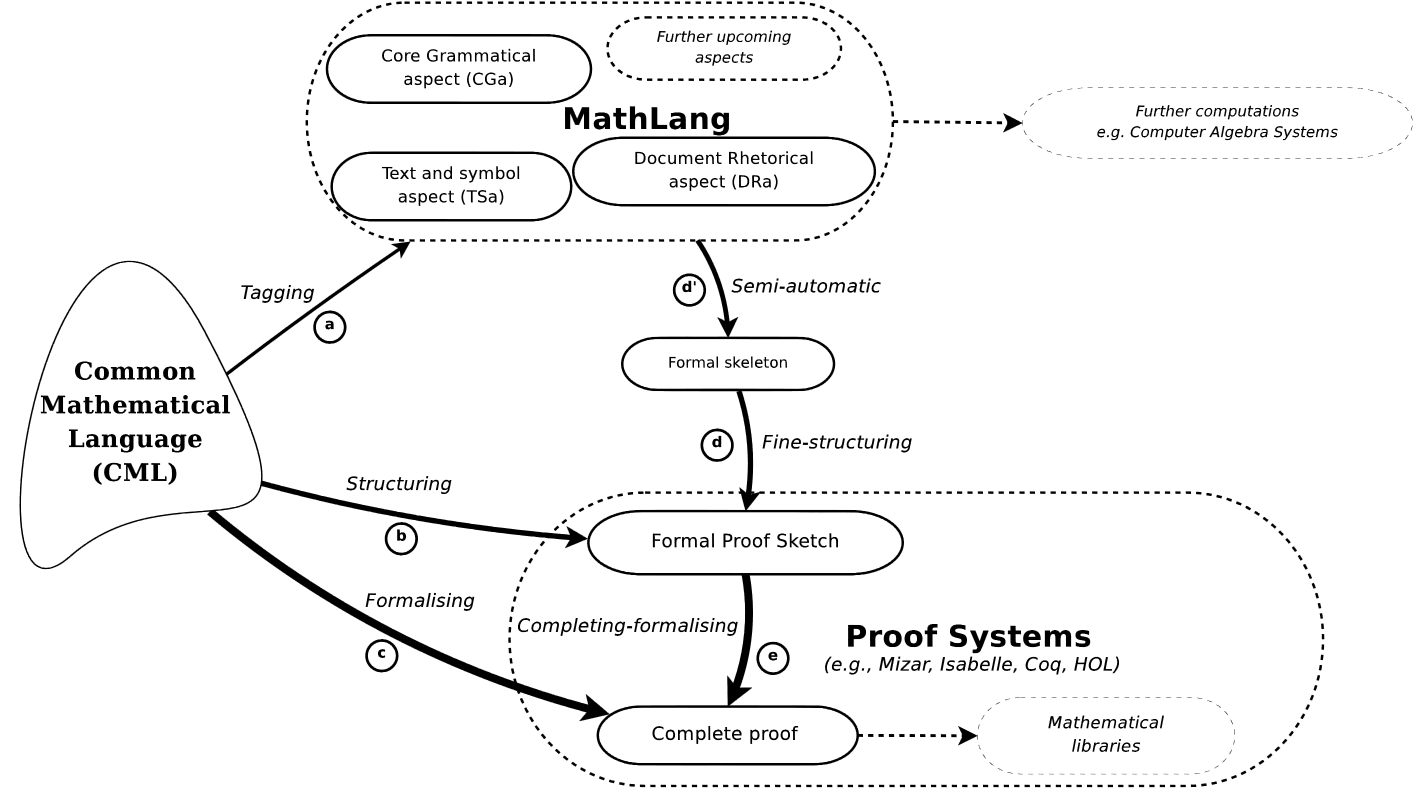
\includegraphics[scale=0.255]{Figures/Background/mathlang.png}
\end{center}
\caption{The MathLang approach to computerisation/formalisation \cite{mathintomizar}\label{fig:mathlang}}
\end{figure}

Figure \ref{fig:mathlang} shows the overall situation of work in the current MathLang Framework.
The labelled arrows show the computerisation paths from the common mathematical language to any proof system. 
The width of the arrow representing each path segment increases according to the expertise required. The level of expertise needed to computerise a CML text straight into a complete proof is very high, however the level of expertise is much smaller by using the \gls{math} framework to help form a formal skeleton and then into a complete proof. The dashed arrows illustrate further computerisation that one can envision.


\subsection{Detailed information on CGa}
\label{subsec:cga}
The current \gls{cga} in MathLang uses a finite set of grammatical \textit{categories} to identify the 
structure and common concepts used in mathematical texts. The aims of the \gls{cga} is to make explicit 
the grammatical role played by the elements of mathematical texts and to allow the validation of the grammatical and reasoning 
structure within the \gls{cga} encoding in a mathematical text. The \gls{cga} checks for grammatical correctness and finds errors like 
an identifier being used without and prior introduction or the wrong number of arguments being given to a function \cite{krzysztofphd}.

\todo[inline]{more detail on dra and cga}
------------------------------------------

\begin{itemize}
\item Reference Zenglars quote

\item Weak type theory into CGa

\end{itemize}

\subsection{Detailed information on DRa}
\label{subsec:dra}

The Document Rhetorical aspects checks that the correctness of the reasoning in the mathematical document is correct and that there are no loops. The \gls{dra} mark-up system is simple and more concentrated on the narrative structure of the mathematical documents whereas other previous systems (such as DocBook \footnote{http://www.docbook.org}, Text Encoding Initiative \footnote{http://www.tei-c.org/index.xml}, OMDoc \footnote{http://www.omdoc.org}) were more concentrated on  the subtleties of the documents. It is used to describe and annotate chunks of texts according to their narrative role played within the document \cite{krzysztofphd}. Using the \gls{dra} annotation system we can capture the role that a chunk of text imposes on the rest of the document or on another chunk of text. This leads to generating dependency graphs which play an important role on mathematical knowledge representation. With these graphs, the reader can easily find their own way while reading the original text without the need to understand all of its subtleties. Processing \gls{dra} annotations can flag problems such as circular reasoning and poorly-supported theorems.
--------------------------------------------------------

\begin{itemize}
\item relations

\item instances

\item Dependency and goto graph
\end{itemize}

\subsection{Detailed information on skeletons}

\begin{itemize}
\item General Proof Skeleton

\item Half baked proof

\item Filled in skeleton
\end{itemize}

\subsection{information on TSa}
\label{subsec:tsa}

The \gls{tsa} builds the bridge between a mathematical text and its grammatical interpretation. The \gls{tsa} is a way of rewriting parts of the text so they have the same meaning. For example some mathematicians may prefer to write "a=b and b=c and c=d", others may prefer "a=b, b=c, c=d" and some others may prefer "a=b=c=d". As you can see all these methods of writing have the same meaning however some symbols are different. The \gls{tsa} annotates each expression in the text with a string of words or symbols which aim to act as the mathematical representation of which this expression is. This allows everything in the text to be uniform.

\subsection{A full worked examples in mathlang}

show step by step translation of mathematical text into isabelle from laamars phd thesis.

\subsection{Conclusion}

\section{Formal Methods and Languages}
\label{sec:formalmethodsandformallanguages}

Formal methods are usually used to assist in formalising in a variety of texts including systems, software and even language itself.

\begin{defin}[Formal Language]
A language designed for use in situations in which natural language is unsuitable, as for example in mathematics, logic, or computer programming.\footnote{www.dictionary.com/browse/formal-language}
\end{defin}

\begin{defin}[Formal Specification]
The specification of a program's properties in a language defined by a mathematical logic.\footnote{www.wiki.c2.com/?FormalSpecification}
\end{defin}

\begin{defin}[Formal methods]
Mathematical approaches to software and system development which support the rigorous specification, design and verification of computer systems.\footnote{www.fmeurope.org/?page\_id=2}
\end{defin}

Formal methods are mathematical approaches to software and system development which support the rigorous specification, design and verification of computer systems \cite{fmeurope}. Specifications are a collection of statements describing how a proposed system should act and function. Formal specifications use notations with defined mathematical meanings to describe systems with precision and no ambiguity. The properties of these specifications can then be worked out with more confidence and can be described to the customers and other stakeholders. This can uncover bugs in the stated requirements which may not have found in a natural language specification. With this, a more complete requirements validation can take place earlier in the development life-cycle and thus save costs and time of the overall project. The rigour using formal methods eliminates design errors earlier and results in substantially reduced time \cite{benefitsofform}. 

\subsection{A brief history of formal methods}

The first known formal language is thought to be used by Frege in his Begriffsschift (1879), Begriffschift meaning `concept of writing' described as `formal language of pure thought'. Frege formalised propositional logic as an axiomatic system.

Formal methods then grew in the following:

\begin{itemize}
\item 1940's, Alan Turing annotated the properties of program states to simplify the logical analysis of sequential programs

\item 1960's Floyd, Hoare and Naur recommended using axiomatic techniques to prove programs meet their specification.

\item 1970's Dijkstra used formal calculus to aid development of non-deterministic programs
\end{itemize}

Formal methods are used today are just as important as when they were used before. Formal methods have a large presence in academia and have also made their way into various industries to prevent design flaws in high integrity systems. Previous design errors have been found in systems such as the Therac-25 machine, which was used for radiation therapy produced by Atomic Energy of Canada Limited in 1982. It was involved in multiple incidents in which patients were give massive overdoses of radiation \cite{baase2003gift}. Another major fault which led to disastrous results was NASA’s Checkout Launch and Control System (CLCS) cancelled 9/2002 \footnote{www.spaceref.com/news/viewnews.html?id=475}.

\subsection{Types of formal methods}


Today there are many different types of formal methods used both in industry and academia. Specification languages are expressive languages with general proof methods, such as VDM, Z, B. Another type of formal method could be program correctness proofs which associates logical inference rules with programming syntax, e.g. Hoare triples and Gries Methodology.There may also be model based approaches to formal methods, which are domain specific languages with precise algorithms for correctness proofs, e.g. Temporal logic \cite{uwa}, Fuzzy logic.  

Formal methods are used to precisely communicate specifications and the function of programs. They are also used to ensure the correctness of systems particularly safety critical systems.

Formal methods have been a success in a variety of projects. For example, in the Sholis project \cite{sholis}, using a formal specification was most effective for fault finding, therefore if the specifications are correct, then the program implemented should then in turn contain less errors if it follows the correct specification.
King, Hammond, Chapman and Pryor's paper \cite{sholis} was based on the SHOLIS defence system. It highlighted the importance of having a formal specification on a system to check for errors. It was found that the Z proof was the most cost effective for fault finding. The Z specification found 75\% of the total faults for the system. Since Z specifications are important for finding faults in SIL4 systems (based on the Sholis project), then checking the correctness of the Z specification is itself very important. Note that the specifications found 75\% of errors and not 100\%. As human error can still occur in formal specifications, using the ZMathLang approach may increase the percentage of errors found.

Another case study where formal methods have been used in industry is the NASA’s Mars Science Laboratory Mission (MSL) \cite{DBLP:journals/corr/abs-1003-1682}. This system relied on various different mechanisms to command the spacecraft from earth and to understand the behaviour of the rover and spacecraft itself. The paper suggested that "\textit{test engineers cannot “eyeball”
the hundreds of thousands of events generated in even short tests of such a complex system}". Therefore runtime verification using formal specification offered a solution to this problem.

A paper reflecting on industry experience with proving properties in SPARK \ref{DBLP:conf/itp/ChapmanS14}, describes a programming language and verification system that will offer sound verification for programs. It states that SPARK and the use of proof tools remain a challenge (published in 2014) as the `adoption hurdle' is perceived too high. Customers and regulators have taken a variety of stances on static analysis and theorem provers. Where some places in industry have adopted the idea others remain sceptical. Hopefully this thesis will present an idea on how formal analysis could be simplified and broken up into smaller more understandable steps and thus would allow more users to take on the idea.

Despite these advantages some managers sometimes argue the cost of producing a system using formal methods do not cover the costs. However the rigour using formal methods eliminates design errors earlier and results in substantially reduced time. Investing more effort in specifying, verifying and testing will benefit software projects by reducing maintenance costs, higher software reliability and more user-responsive software \cite{chantatub}.

So far we have seen what are the different types of formal methods, where formal methods have been used, and why some people are still reluctant to use them. So what needs to be done to make “formal methods” industrial strength? Nirmal Pandey \cite{formalmethodslides} suggests the following: 

\begin{itemize}
\item Bridge gap between real world and mathematics
\item Mapping from formal specifications to code (preferably automated)
\item Patterns identified
\item Level of abstraction should be supported
\item Tools needed to hide complexity of formalism
\item Provide visualization of specifications 
\item Certain activities not yet ‘formulizable’ methods
\item No one model has been identified which should be used for software)
\end{itemize}


\subsection{Conclusion}

In this section we have identified the differences between formal methods, formal languages and formal specification. We have seen how formal methods originated from mathematics and how it grew over time to become what it is today. We see a connection with Frege's work on mathematical notation and identified it as the first formal notation found in history. We identified there are a variety of formal methods and new methods are even being developed today to comply with the systems in questions. For example MSL had it's own specification language developed for the system in order for the system to be verified. Despite all the advantages, some managers are still reluctant to use formal methods in their system development and thus as Pandey suggested there still needs to be some work done on making formal methods industrial strength. One of his suggestions was that tools are needed to hide complexity of formalisms and to provide visualization of specifications, which this thesis addresses.

\section{Z Syntax and semantics}
\label{sec:theznotation}

In this section we give a brief overview on the core fundamentals of the Z formal language. We outline a basis of propositional and predicate logic and describe how Z syntax is formed to specify a system.

\subsection{Introduction to Z}


Z is based on predicate Calculus, Zermelo-Frankel set theory as we introduced at the beginning of this chapter in section \ref{subsec:rftb}.

It is a particular formal method which was developed to specify the new Customer Information Control System (CICS) functionality \cite{cics}. The set theory includes standard set operators, set comprehensions, Cartesian products and power sets. Z also has other aspects such as schemas which are used to group mathematical objects and their properties. The schema language can be used to describe the state of a system and ways in which that state may change \cite{Woodcock:1996:UZS:235337}.

\subsection{Propositional and predicate logic}

Z specifications are built using predicate and propositional logic.

\subsubsection{Propositional logic}

Propositional logic works with statements which must be either true or false but can not be both. The following are propositional statements:
\begin{itemize}
\item A tree is green

\item A tree has leaves

\item All plants have flowers
\end{itemize}

Propositions can be connected in a variety of ways. Figure \ref{tab:logcon} shows a table of logical connectors in order of operator precedence.

\begin{table}[H]
\centering
\begin{tabular}{| c | c | c |}
\hline
$\neg$ & negation & \textbf{not} \\
\hline
$\land$ & conjunction & \textbf{and} \\
\hline
$\lor$ & disjunction & \textbf{or} \\
\hline
$\implies$ & implication & \textbf{implies} \\
\hline
$\Leftrightarrow$ & equivalence & \textbf{if and only if} \\
\hline
\end{tabular}
\caption{Logical connectors giving the symbol, its name and pronunciation. \label{tab:logcon}}
\end{table}

We can now build compound propositions, which are propositional statements joined together using these connectors, e.g.

\begin{itemize}
\item the glass is full $\land$ the glass is clear

\item the phone isn't working $\lor$ the phone battery has died

\item the sun is shining $\implies$ I don't need a raincoat
\end{itemize}

\subsubsection{Predicate logic}

Predicate logic allow us to make statements which describe properties that must be satisfied by every, some or no objects in some universe of discourse. Examples are:

\begin{itemize}
\item Every plane can fall out of the sky.

\item At least one cloud has a silver lining.

\item Jake knows all rugby players in the Scottish team.
\end{itemize}

To formalise such statements we require a language of predicate calculus. A predicate is a statement with a place for an object. A predicate can turn into a proposition once we put an object in it, therefore we can not say whether it is true or false once the predicate has filled in mission information. For example we can say `$x > 5$' is a predicate but not a proposition until we know what `$x$' is. We can make a proposition out of `$x > 5$' by putting a \textit{quantifier} with it. So we can say, `there is an $x$ which is larger than 5'. This is written formally as `$\exists x > 5$'. This statement can now be written in our Z syntax.

We can now formalise one of our previous predicate statements:
\newline
$\exists c: CLOUD @ c\ has\ silver\ lining$
This statement says that there exists $c$ which is a cloud and $c$ has a silver lining.

\subsection{Sets and Types}

A \textit{set} is a collection of distinct objects called \textit{elements}. For example the set of all people. Every expression in a Z specification belongs to a set called its \textit{type} and whenever we introduce a variable we must declare its type \cite{essenceofz}. For example:

\begin{zed}
[HUMAN]\ the\ set\ of\ all\ humans \\
\nat\ the\ set\ of\ all\ natural\ numbers
\end{zed}

Another way of introducing types is using a \textit{free type definition}, where once enumerates the names of the elements in that type, for example:

\begin{zed}
SHAPES ::= square | circle | triangle \\
PLANTS ::= tree | shrub | herb \\
\end{zed}

In Z specification, we introduce variables before they are used in the expressions (predicates) by a means of writing a \textit{declaration}. A declaration can introduce either one or multiple variables. For example:

\begin{zed}
ralph: HUMAN \\
a, b, c: \nat
\end{zed}

\subsection{Structure of a Z specification}

In the Z notation there are two languages: the mathematical language and the schema language. The mathematical language is used to describe various aspects of a design: object, and the relationships between them. The schema language is used to structure and compose descriptions: collecting pieces of information and naming them for re-use. A schema consists of two parts: a \emph{declaration part} and a \emph{predicate part}. The \emph{declaration part} consists of declared variables and the \emph{predicate part} describes the variable values. We can write a schema either horizontally (figure \ref{fig:horizontalschema}) or vertically (figure \ref{fig:verticalschema}).

\begin{figure}[H]
\vspace{-0.2in}
\centering
\begin{minipage}{0.45\textwidth}
\begin{zed}
\noindent Schema\ Name \defs [declarations | predicates]
\end{zed}
\vspace{-0.18in}
\caption{An example of a schema written horizontally.\label{fig:horizontalschema}}
\vspace{-0.2in}
\end{minipage}\hfill
\begin{minipage}{0.45\textwidth}
\begin{schema}{Schema\ Name}
declarations
\where
predicates
\end{schema}
\vspace{-0.2in}
\caption{An example of a schema written vertically. \label{fig:verticalschema}}
\vspace{-0.2in}
\end{minipage}
\end{figure}

If we wanted a property of some system which consists of two variables $x$ and $y$ and state that $x$ must be smaller than $y$ then we can write:

\begin{schema}{xLessThany}
x: \nat \\
y: \nat
\where
x < y
\end{schema}

We can also introduce global variables by means of an \textit{axiomatic description} in Z. These global variables may be referred to throughout the specification. An example this Z construct is as follows:

\begin{axdef}
k: \nat \\
\where
k = 100
\end{axdef}

With this axiomatic description in place within the Z specification means that whenever the global variable $k$ is referred to, it will always represent the natural number 100.

The full language of Z can be explored in \cite{spiveyreferencemanual}, \cite{essenceofz} and \cite{Woodcock:1996:UZS:235337}.

\subsection{A full example in Z}
Here is a small schema which tells a story about a child called Ralph and his mum. We declare the types $OBJECT$ which is a type containing all objects. We also declare the type $EMOTION$ which consists of 3 emotions: $happy$, $sad$ and $angry$

\begin{zed}
[OBJECT] \\
EMOTION::= happy | sad | angry
\end{zed}

In this first schema we declare the state variables which is ralph and mum who are of type human, colourIn which maps a human to an object (representing that particular human is colouring in that object) and feeling which maps a human to an emotion (representing that human is feeling that emotion).

In the state we say that ralph is always feeling happy
\begin{schema}{ColouringIn}
ralph, mum:HUMAN \\
colourIn:(HUMAN \pfun OBJECT) \\
feeling:(HUMAN \pfun EMOTION)
\where
feeling(ralph \mapsto happy)
\end{schema}

In this schema we say that when ralph is colouring in a picture, mum is feeling happy. We use a $\Delta$ to signify this schema changes the current state.
\begin{schema}{ColourPicture}
\Delta ColouringIn \\
picture: OBJECT 
\where
colourIn(ralph \mapsto picture) \\
feeling(mum \mapsto happy)
\end{schema}

However in this schema, we say we say when ralph is colouring the wall, then mum is angry.
\begin{schema}{ColourWall}
\Delta ColouringIn
wall: OBJECT \\
\where
colour(ralph \mapsto picture) \\
feeling(mum \mapsto angry)
\end{schema}

\subsection{Conclusion}

In this section we gave a brief introduction to Z what it is made up of. We give a short overview of propositional and predicate logic as well as defining the structure of a Z specification. We give a full example of a Z specification and explain each part and what it means. In the next section we identify various proving systems which currently exist for mathematics, other formal methods and Z.

\section{Proving systems}

Before the day's of mechanical computers the only way to check a mathematical documents logic was correct was using hand written proofs. Then one can ask another mathematician such as a peer or an expert in the field to check over ones mathematics to prove it was correct. However even with more than one mathematician checking over the mathematical logic, one could not be 100/% certain it was correct due to human error. 

Once mechanical computers were developed, work started on proof assistants (or proof checkers) and automated theorem provers. Checking the correctness using automated theorem provers adds an extra level it also adds a level of certainty that the mathematics written is correct, thus it is a good idea to check the correctness of systems which are or high integrity.

\subsection{Levels of Rigour}

Depending on the integrity of the system being developed there are various formal techniques which could be used to mathematically verify the system design and implementation satisfy the functional and safety properties. These specifications and verifications may be done using various degrees of rigour such as:

\begin{itemize}
\item Level 1 represents the use of mathematical logic to specify the system.
\item Level 2 uses pencil-and-paper proofs.
\item Level 3 consists of formal proofs being checked by a mechanical theorem prover.
\end{itemize}

Level 1 can be done using various levels of abstract to describe the system. One abstract level would be to describe the abstract properties of the system and another abstract level could be to describe the implementation in an algorithmic way.

Level 2 goes beyond level 1 in that the pencil-and-paper proofs are used to describe that the lower level properties imply the abstract properties in level 1.

Level 3 is the highest level of rigour one can do to check the proofs of a specification. It consists of using an autonomic theorem prover to confirm that all proofs are valid. The level 3 process of convincing a mechanical prover is really a process of developing an argument for an ultimate sceptic who must be shown every detail \cite{encyclopedia}.

\subsection{Proving systems for maths}

In section \ref{subsec:rftb} we saw how mathematics has evolved and become the complex system it is today. Since the rise of computers the ability to check some of these old and new theories automatically has been possible.

Mizar \cite{mizar}, Isabelle \cite{isabelle} and Coq \cite{coq} are types of \textbf{Proof assistants} (or proof Checkers). Whilst PVS and Vampire are types of \textbf{theorem provers}. Both proof assistants and theorem provers can be classed as `proof systems'.
Each proof system provides it's own formal language for writing mathematics based on some foundation of logic.

The first project which used a `computer' for automated verification dates back to 1967. N.G. de Bruijn started the AutoMath Project (described in section \ref{subsec:rftb}). A few years Later Trybulec created his project Mizar \cite{mizar}, where he aimed to develop a computerised assistant to edit mathematical papers.

From 1989 the works of the Mizar project worked on improving the Mizar system and developing the database for mathematics. The Mizar Language is a formal language which is derived from the mathematical vernacular. The author wanted to design a language readable for mathematics and rigorous enough to enable processing and verifying by computer software.

\begin{figure}[H]
\begin{center}
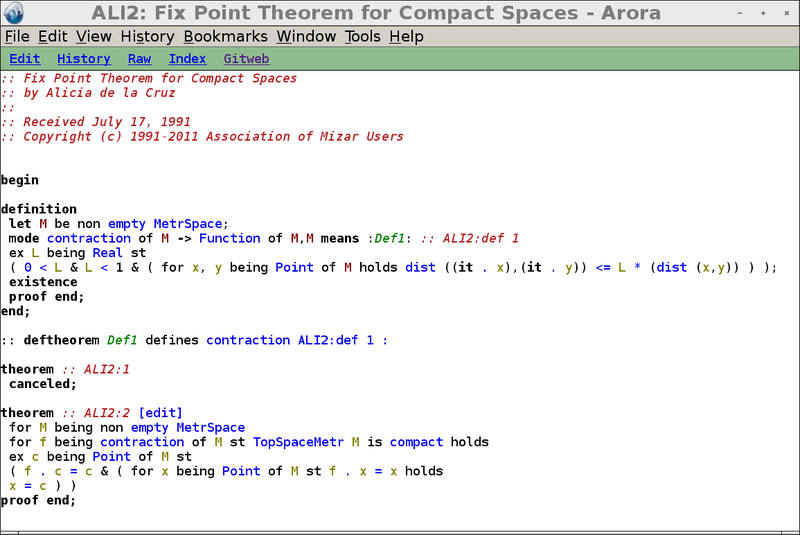
\includegraphics[scale=0.5]{Figures/Background/mizar.png}
\end{center}
\caption{Screenshot of the Mizar theorem prover \cite{mizar}. \label{fig:mizar}}
\end{figure}

Isabelle \cite{isabelle} is a generic proof assistant. It accepts a variety of mathematics into it's syntax and also has it's own formal language and provides tools for those formulas in a logical calculus. The main application if the formalization of mathematical proofs and formal verification which includes proving the correctness for computer hardware or software.

\begin{figure}[H]
\begin{center}
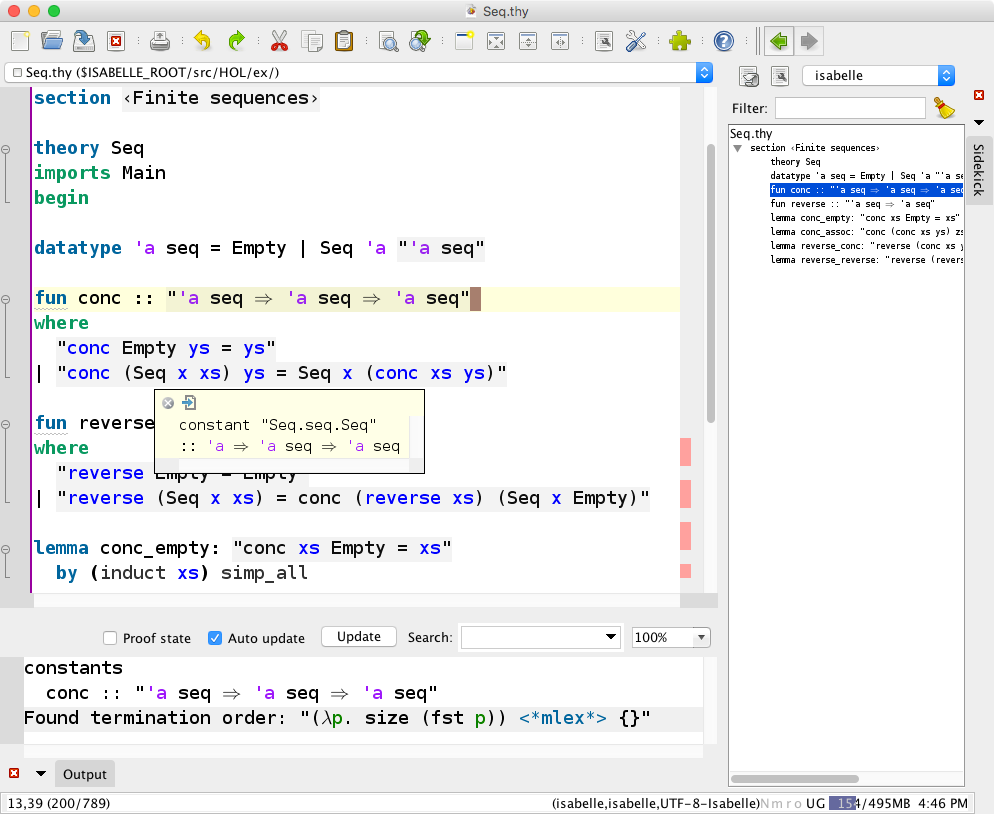
\includegraphics[scale=0.4]{Figures/Background/isabelle.png}
\end{center}
\caption{Screenshot of the Isabelle theorem prover \cite{isabelle}. \label{fig:isabelle}}
\end{figure}

A third proof assistant is Coq \cite{coq}, which also provides it's own formal language to write mathematical definitions, executable algorithms and theorems for semi-interactive development of machine checked proofs. Although it names itself a 'formal proof management system', like Isabelle and Mizar it is used to verify and check properties of software and hardware systems and the formalization of mathematics.

\begin{figure}[H]
\begin{center}
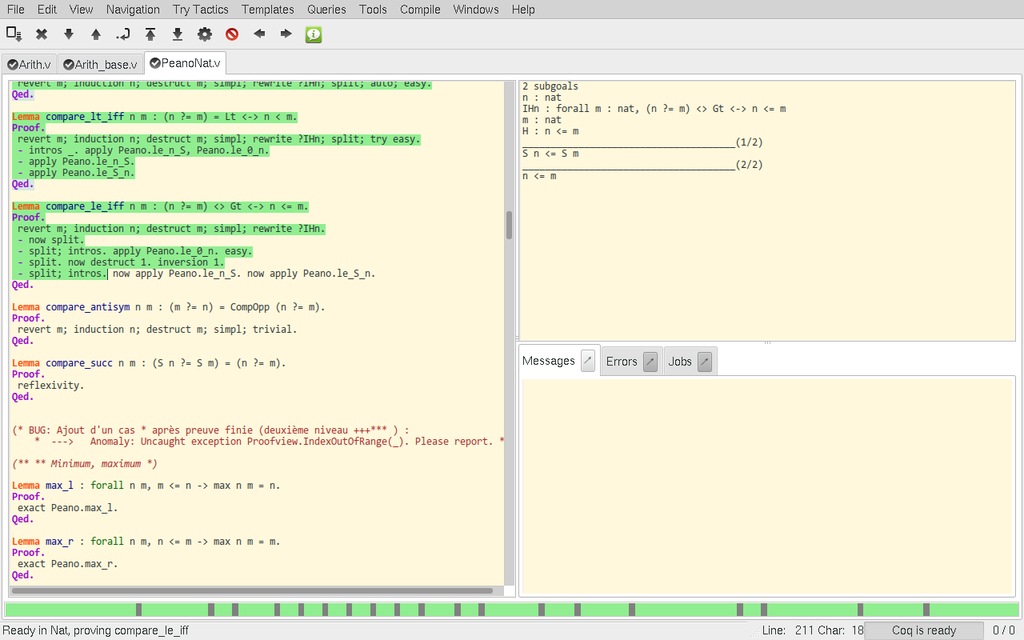
\includegraphics[scale=0.4]{Figures/Background/coq.png}
\end{center}
\caption{Screenshot of the Coq theorem prover \cite{coq}. \label{fig:coq}}
\end{figure}

There are many other proof assistants for general mathematics (Nuprl, Otter etc.) and generally they all support checking for correctness of mathematical theories. However, a disadvantage of using these systems is the enormous expense of formalisation in any proof system. 

A mathematician who wants to verify the logic of a document has to decide on a proof system to use. All proof systems have their own advantages and disadvantage as well as the mathematician then needs to learn and create a document with the syntax of his chosen proof system.

Also, not all proof system have meaningful support for the common mathematical language or a generic formal specification language. There may be proof systems built for specific formal specification language but not one which supports all. The rigid structure and rules for formal documents created in proof systems are more closer to a computer programming language then to natural language. An exception of this is Mizar, however even natural language written in Mizar has to be structural and rigid.

In summary, computerising a any form of mathematical document using a proof system is similar to writing a computer program. Where the formal language of the proof system corresponds a programming language. Therefore, mathematicians require to have some form of computer programming knowledge. A proof system can check the logical correctness of a document if it detailed enough for the software to parse, therefore the computerisation of the mathematical document becomes labour intensive and tedious for the author to write.

\subsection{Proving systems for specific formal method}


Dafny \cite{dafny} features modular verification, so that the separate verification of each part of the program implies the correctness of the whole program. This is similar to \gls{zmath}, where Dafny checks different parts of the text and thus confirms correctness of the full text, \gls{zmath} checks the correctness of the text through different levels of rigour to imply and fully correct specification.

Dafny was able to do a proof for the Schorr-Waited Algorithm, however the writer states that the loop invariants are complicated because they are concrete. A refinement approach such as Jean-Raymond Abrials \cite{abrial} may be preferred in this case.  

Another attempt at checking for correctness was written by Rex L.Page in Engineering Software Correctness \cite{engineeringsoftwarecorrectness}. A general theme within this paper, is that design and quality are important in engineering education. When teaching students how to create programs, it is not enough just to teach them how to develop software but to how develop good quality software. This paper describes experiments with the use of ACL2 (a subset of lisp), which is embedded on mechanical logic to focus on design and correctness. Using ACL2 emphasises the importance of software design and correctness. 

ALC2 is coded therefore users must know how to code software to formulate proofs. The intention of \gls{zmath} is to allow many people in the development team to be able to formulate proofs such as project managers, designers, engineers etc. Therefore no coding is necessary and no new programming language is needed.

PVS (Prototype Verification System) \cite{pvs} is an environment for constructing specifications and developing proofs which have been mechanically verified. PVS has it's own specification language, which engineers would need to learn as well as using the environment for proofs. Type checking is undecideable for the PVS type system. The PVS also provides a language for defining high-level inference strategies.


\subsection{Proving Systems specific for Z}
\label{subsec:provingSystemsForZ}

A tool which analysis the Z notation is Hol-Z \cite{hol-z}, which is also a proof environment for Z. Hol-Z is embedded in Isabelle/HOL therefore it provides a Z type checker, documentation facilities and refinement proofs with a theorem prover. The Z specification is implemented in \LaTeX{} then typed checked using an external plug in Zeta, it is then transformed into SML files to be added into the Hol-Z theorem prover environment. The user will need to have some good expertise in using the Hol-Z proof environment in order to fully prove the specification.

Fuzz \cite{spiveyfuzz} is another example of a type-checker for the Z language. It includes style files for \LaTeX{} and checks for the logical correctness and Z type correctness of Z specifications. This is different to the \gls{zcga} type checker as the weak types in \gls{zcga} check for the grammatical correctness and not the full logical correctness of Z. Therefore the grammatical correctness of partially formal specification can also be checked. The \gls{zmath} framework presented in this thesis uses the `zed' \LaTeX{} style package to typeset the Z specifications in the documents.

There are many other tools for Z which can be found on the Z Notation Wikia page \cite{zwikia}. For this thesis we will concentrate on translating Z specifications into theorem prover Isabelle \cite{isabelle}. Isabelle is a generic proof assistant which allows mathematical formulas to be expressed in a formal language and includes numerous contributions worldwide. It contains a large mathematical tool-kit (majority of Z can be represented in Isabelle) and has a lot of support in forms of documentation and online. It is distributed for free, easy to find, download and install and is regularly updated. The original \gls{math} has translated mathematical texts into Isabelle already (\cite{mathintoisa}) therefore we can use parts of that research to aid the research in this thesis.

\subsection{Other properties to prove}
\label{subsec:propertiestoprove}

\begin{defin}
A logical formula associated to a correctness claim for a given verification property. The formula is valid if and only if the property holds. The correctness of the property under verification is “delegated” to proving the correctness of the new formula \cite{handbookofembed}.
\end{defin}

Therefore a proof obligation is a logical formula which the specifier must show to be a consequence of the specification so that a specification can be taken to be acceptable. In a more pragmatic sense proof obligations may be viewed as what the developer of a specification is obliged to prove in order to confirm that development is consistent.

Woodcock and Cavalcanti \cite{woodcock2004tutorial} use the alphabetised relational calculus to give denotational sematics to different constructs from programming patterns. This paper describes `\emph{healthiness conditions}' which identifies properties that characterise theories. Each one of these healthiness conditions represents a fact about the computational model for the programs being studied.

\begin{exam}
The variable `\emph{clock}' is an observation of the current time which is always moving onwards. The following predicate `B' specifies the clock variable:

\begin{zed}
B \defs clock \leq clock'
\end{zed}
\end{exam}

The healthiness condition described in this paper are specific proof obligations for the concept of \gls{utp}. The semantic model of \gls{utp} is presented a Z specification. Therefore the healthiness conditions for the specification would in one way be checking for the correctness of the \gls{utp} model. In a similar way, it is important to add healthiness conditions or as we call them in this thesis, `safety properties' in order to check each individual specification for various types of correctness.

Stepney describes two proof project written in Z in her paper a tale of two proofs \cite{stepney1998tale}. She explains how the proof process is deeply affected by \textbf{why} something is being proved, \textbf{what} is being proved and \textbf{how} the finished proof is to be presented. Stepney suggests that the proofs for specifications themselves do not have to be deep but the workings of what to proves can add to the labour. It is also important to keep in mind how deep the customer wants the proof and what level of assurance they need. She highlights 5 different points to prove:

\begin{figure}[H]
\begin{enumerate}
\item \textbf{Consistency checks}: Prove that your specification is consistent and that it has a model.

\item \textbf{Sanity Checks}: In a `state and operations' style specification, prove that the state invariants are satisfied throughout and that the precondition of each operation is not \emph{false}.

\item \textbf{Emergent properties of a single specification}: Make explicit as a theorem some desired or suspected property of the specification, then prove it holds.

\item \textbf{Required properties of a single specification}: If some property is required to hold of the specification, and the specification has captured it implicitly, it needs to be made explicit and shown to hold.

\item \textbf{Properties across specifications}: Prove that a certain relationship holds between two specification such as the refinement relationship.
\end{enumerate}
\caption{Different points to prove in a specification \cite{stepney1998tale}. \label{fig:ptp}}
\end{figure}

Some of the points in figure \ref{fig:ptp} would be fairly easy to automate such as `consistency checks' and `sanity checks' however the other 3 points would be difficult to automate as they would all depend on the specification in question and would perhaps need some \emph{extra information} to decipher these properties. For example if one wish to automate proof obligations from point 5 the user would need to implement another specification (such as a refinement specification) and then prove the relationship between the original specification and the new one. In this thesis, we will concentrate on properties described in point 1 which have been automated. 

Stepney also explains that if the development process is incremental, it would be worthwhile getting a good structure for a proof up front which you can add more details in later. \gls{zmath}  can automatically generate this first structure which could be added to if needed. It can produce a specification in Isabelle syntax where other properties and details could be added to by the user at a later stage.

Most recently Mark Adams \cite{JFR4576} describes that even formalisation itself can be prone to error and therefore even if we do get a fully proven specification, the proof will also need to be checked. He outlines the flyspeck project which assists with the checking of formalised proofs. Adam calls this `\emph{proof auditing}', which adds another step of rigour to the theorem. \gls{zmath} assists with translating the specification into a theorem prover along with consistency lemmas to prove. The user can then choose to prove these lemmas and the proof audit their theorem. However, even if proof auditing adds another level of rigour it is important to keep in mind who the user is doing the proofs for. As Stepney pointed out in \cite{stepney1998tale}, some clients wouldn't need that amount of rigour for their projects and only the proved safety properties may be enough.

Woodcock et al also describes that a specification can be developed in such a way that can lead to a suitable implementation called refinement \cite{Woodcock:1996:UZS:235337}. 

To refine a formal specification, more data must be added e.g. how certain calculations should be carried out. He states an abstract specification may leave design choices unresolved and its up to the refinement specification to resolve some of these choices. An example of this is shown in the following:

\begin{exam}

\begin{schema}{ResourceManager}
free: \mathbb{F} \nat
\end{schema}

 Any resource that is free can be allocated

\begin{schema}{Allocate}
\Delta ResourceManager \\
r!: \nat
\where
r! \in free \land free' = free \setminus \{r!\}
\end{schema}

\label{exam:allocate} 
\end{exam}

If there is more than one resource free in example \ref{exam:allocate} then this will class the specification as non deterministic.

Example \ref{exam:allocate} can be refined in that if there is more than one resource free, the resource with the lowest number should be allocated. This is shown in the following example:

\begin{exam}

\begin{schema}{Allocate}
\Delta ResourceManager \\
r!: \nat
\where
r! \in min~free \land free' = free \setminus \{r!\}
\end{schema}
\label{exam:allocaterefine} 
\end{exam}

Refining an abstract specification which is described in \cite{Woodcock:1996:UZS:235337} and in \cite{spiveyreferencemanual} is exactly what Stepney points out in point 5 from figure \ref{fig:ptp}. To show that this property holds the user would need to produce another specification which refines their original one and then include properties of how they relate to each other. Since each individual specification is different then refinement specifications would be different to. Thus we wouldn't be able to automate this point. \gls{zmath} aims to assist the user in translating and proving their specification, the proof effort will be focused on properties which can be automated e.g. item 1 in figure \ref{fig:ptp}. Items 3, 4 and 5 would be to difficult to automate and therefore out of the scope of this thesis.

Fraser and Banach \cite{DBLP:conf/sefm/FraserB07} state that model based formal methods usually come in the form of many incompatible tools. Therefore they devised a system to combine different techniques called the frog toolkit.

Many verification tools today tend to utilize a single technique and are unable to interact easily with other tools in other kits. A more dynamic approach such as RODIN \cite{Jones05j} and Overture \cite{overture} are perusing a more flexible approach. \gls{zmath} will need to follow in the footstep of these two tool-kits in order to be successful and not commit to a particular system until needed. This is why the steps 1-3 of the translation path (figure \ref{fig:steps}) are generic and can be used to translate the specification in any theorem prover. It is only at step 4 which is where we start committing to Isabelle.

The main aim of the frog tool-kit was to support retrenchment, which is a formal technique used along side refinement. The new tool-kit was created which was able to use a variety of techniques in a single working environment. The frog tool-kit can prove the relationships between multiple specifications (which we see as point 5 in figure \ref{fig:ptp} from Stepney \cite{stepney1998tale}). To do this the user should have at least 2 specifications implemented to prove the relations (usually one is a refinement specification of the first one). These specifications where then written in frog-ccc, a meta language to use within the frog tool-kit. \gls{zmath}'s aim is to prove the properties described as point 1 in figure \ref{fig:ptp} therefore another specification to refine the abstract one is not needed.

Since formal specifications are not executable it is difficult to verify the consistency of the specification. Wen, Miao and Zeng \cite{DBLP:conf/icsea/WenMZ06} present and approach to generate proof obligations to check for consistency of object Z specifications. Checking for consistency of specifications is described in point 2 in figure \ref{fig:ptp}. In their paper, the authors explain two 
types of proof obligations which check that a object Z specification is non conflictive. They are:

\begin{itemize}
\item Existence of initial state

\item Feasibility of an operation
\end{itemize}

The initial state is a state within the state space of the specification which should exist and satisfy the stateInvariants. In all specifications their should exist a state which initialised the beginning state of the specification.

An operation can transform one state to another. Therefore if the operation is feasible, the pre state (state before the state change) and post state (state after the state change) should always satisfy the state invariant. 

We will use the definitions shown in \cite{DBLP:conf/icsea/WenMZ06} to automatically generate the proof obligations to check for the correctness of our Z specifications as the specifications we use in this thesis are all state based.

In summary there are many different approaches to finding properties to prove about formal specifications. Some which can be easily automated, some which need some more information and some which will need to be written manually. Since we do not expect the users of \gls{zmath} to be experts in the fields of theorem proving we want to attempt to automate proof obligations which can be easily understood by the user. Then once the user gains some knowledge of their theorem prover, they can add other proof obligations manually. As explained in this section, it is important to note who the user is doing the proofs for, as the customer may not need or want complex proofs. Therefore we shall generate the proof obligations which can be automated and do not require any extra information to be automated.


\subsection{Conclusion}

\todo[inline]{Write conclusion to proving systems}

\section{Background Conclusion}

\subsection{MathLang for Z}

\todo[inline]{Write conclusion to background chapter}

\begin{itemize}
\item \cite{fmpresetation} states what ro do to make formal methods industrial strength

\item \cite{lamarphd} stating in future work mathlang should be developed to cope with more mathematics (formal spec is a type of mathematics)

\item diagram of math text to theorem prover using mathlang + diagram of specification to theorem prover using mathlang
\end{itemize}

ZMathLang covers items 1, 3, 5, 6, 7 from section \ref{sec:formalmethodsandformallanguages}.